% ********** Chapter 4 **********
\chapter{Solution}
\label{sec:Solution}

There are two kind of connection solution of the core of Web Call, the Relay Call and Third Party Call. The different between them is the way they handle media stream.

The Relay Call Controller works as a back-to-back agent and forwards media streams, while Third Party Call Controller only establishes connections by sending out SIP messages and it does not handles any streams itself. 

\section{Relay Call}
\label{sec:Solution:RelayCall}

\begin{figure}[!hbtp]
\centering
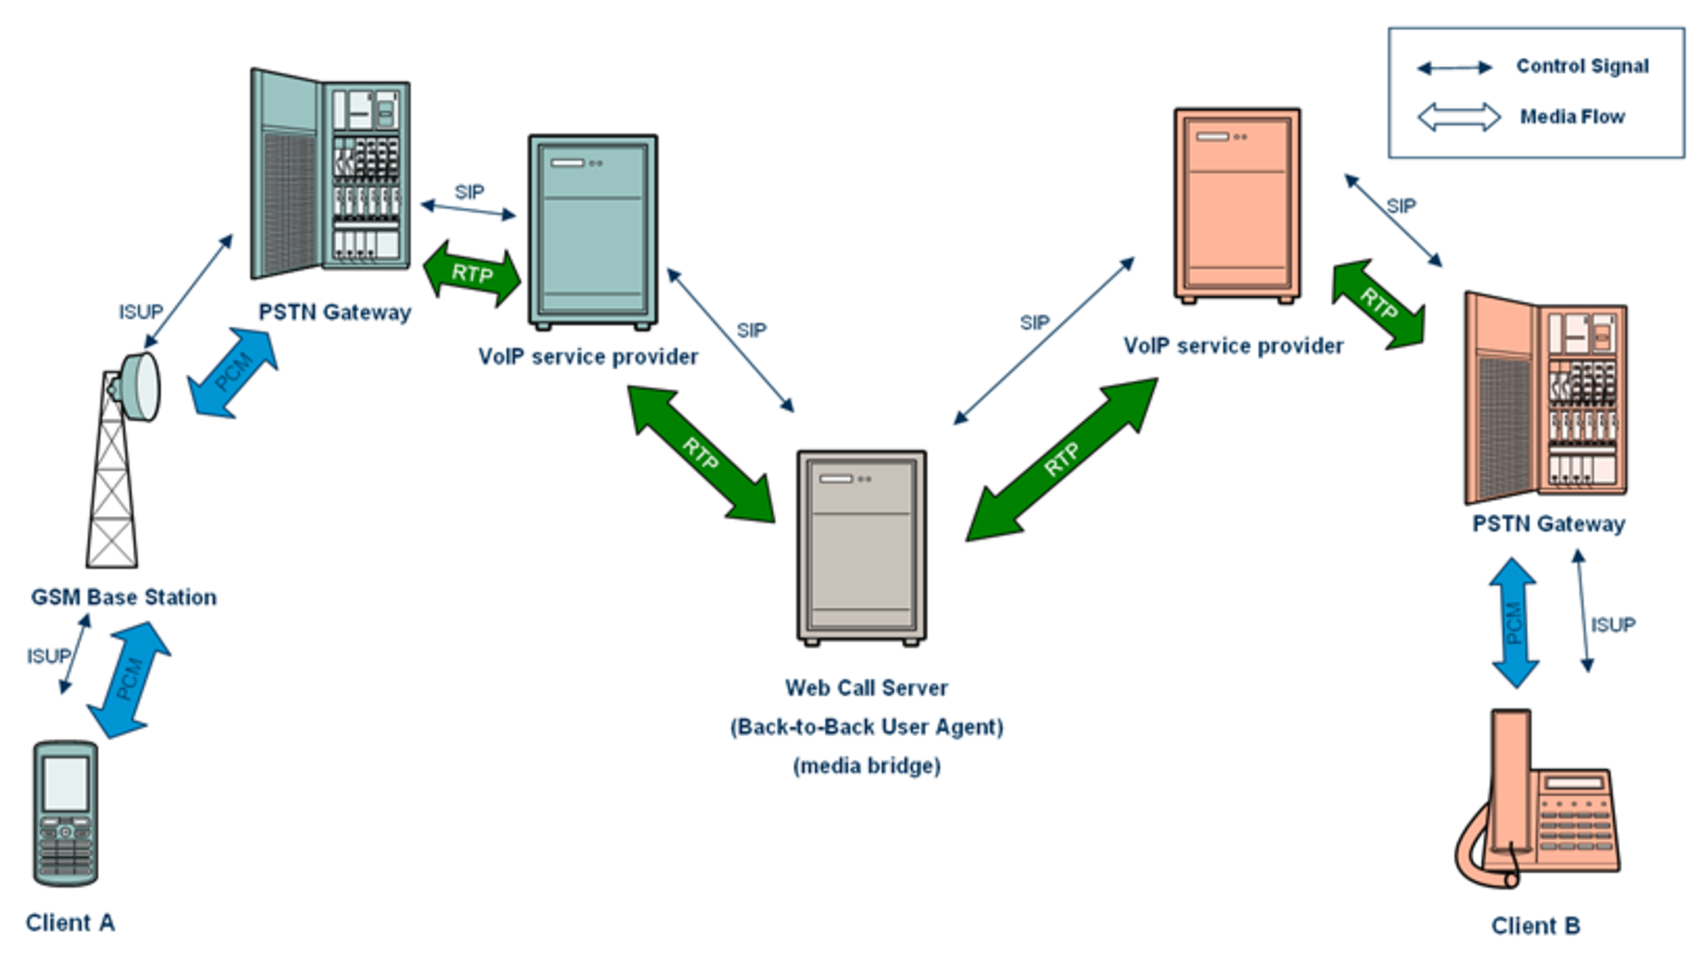
\epsfig{file=chap04/resources/the_signal_and_media_flow_of_relay_call, width=5.34in}
\caption{The signal and media flow of Relay Call}
\label{fig:TheSignalAndMediaFlowOfRelayCall}
\end{figure}

The signal and media flow of Relay Call is shown in Figure \ref{fig:TheSignalAndMediaFlowOfRelayCall}. In this scenario, the Web Call Example Application acts as a back-to-back user agent. It sets up the connection and forwards the media stream. It can be seen from the picture that both signal and media are handled by Web Call Server. When it starts, it try to call client A. After it establishes a session with client A, it will try to call client B and also establish a session with client B. After that, it will work as a media stream bridge and forward media stream from client A to B, as well as from client B to A.

For a detail description and mechanism of Relay Call, please refer to the master thesis of \textbf{Web Call SDK} by \textit{Yuening Chen}\cite{WebCallSDK}.

\section{Problem of Relay Call}
\label{}

\subsection{The load on controller}
 
The controller here acts as a back to back user agent (B2BUA). It receives the RTP flow from one client and transfers it to another client. It does the same in the opposite direction. That means all of the RTP traffic will go through the controller. So the load on controller will be heavier as with the number of concurrent users increases. A powerful host is needed to handle the RTP flows. However the design goal of Web Call SDK was simply a tool kit that can easily be integrated into a web site. Unfortunately, this  current mechanism of session control will decrease the performance of whole web site. 

\subsection{The latency of the phone call}
 
As can be seen from the session flow, the RTP goes from one client to the controller via a SIP provider and then the controller transfers the RTP to another client via the SIP provider again. This means that each direction of RTP will go through SIP provider twice. So the latency of the phone call via the SIP provider will be double that of normal calls.  The latency of phone-to-phone call via Web Call SDK test turned to be more then 2 seconds. It is quite unacceptable. 

\subsection{Lack of Reliability}

Since all of RTP flows go through the controller, thus if the controller crashes, all of calls will be immediately interrupted. 



\section{Third Party Call}
\label{sec:Solution:ThirdPartyCall}

In the traditional telephony context, third party call control allows one entity (which we call the controller) to set up and manage a communications relationship between two or more other parties. Third Party call control (referred as 3pcc) is often used for operator services (where an operator creates a call that connects two participants together) and for conferencing. The signal and media flow in third party call is show in Figure \ref{fig:TheSignalAndMediaFlowOf3pc} The advantage of third party call in Web Call is that the controller only need to handle message transfer and leaves the media flow for the ISP.

\begin{figure}[!hbtp]
\centering
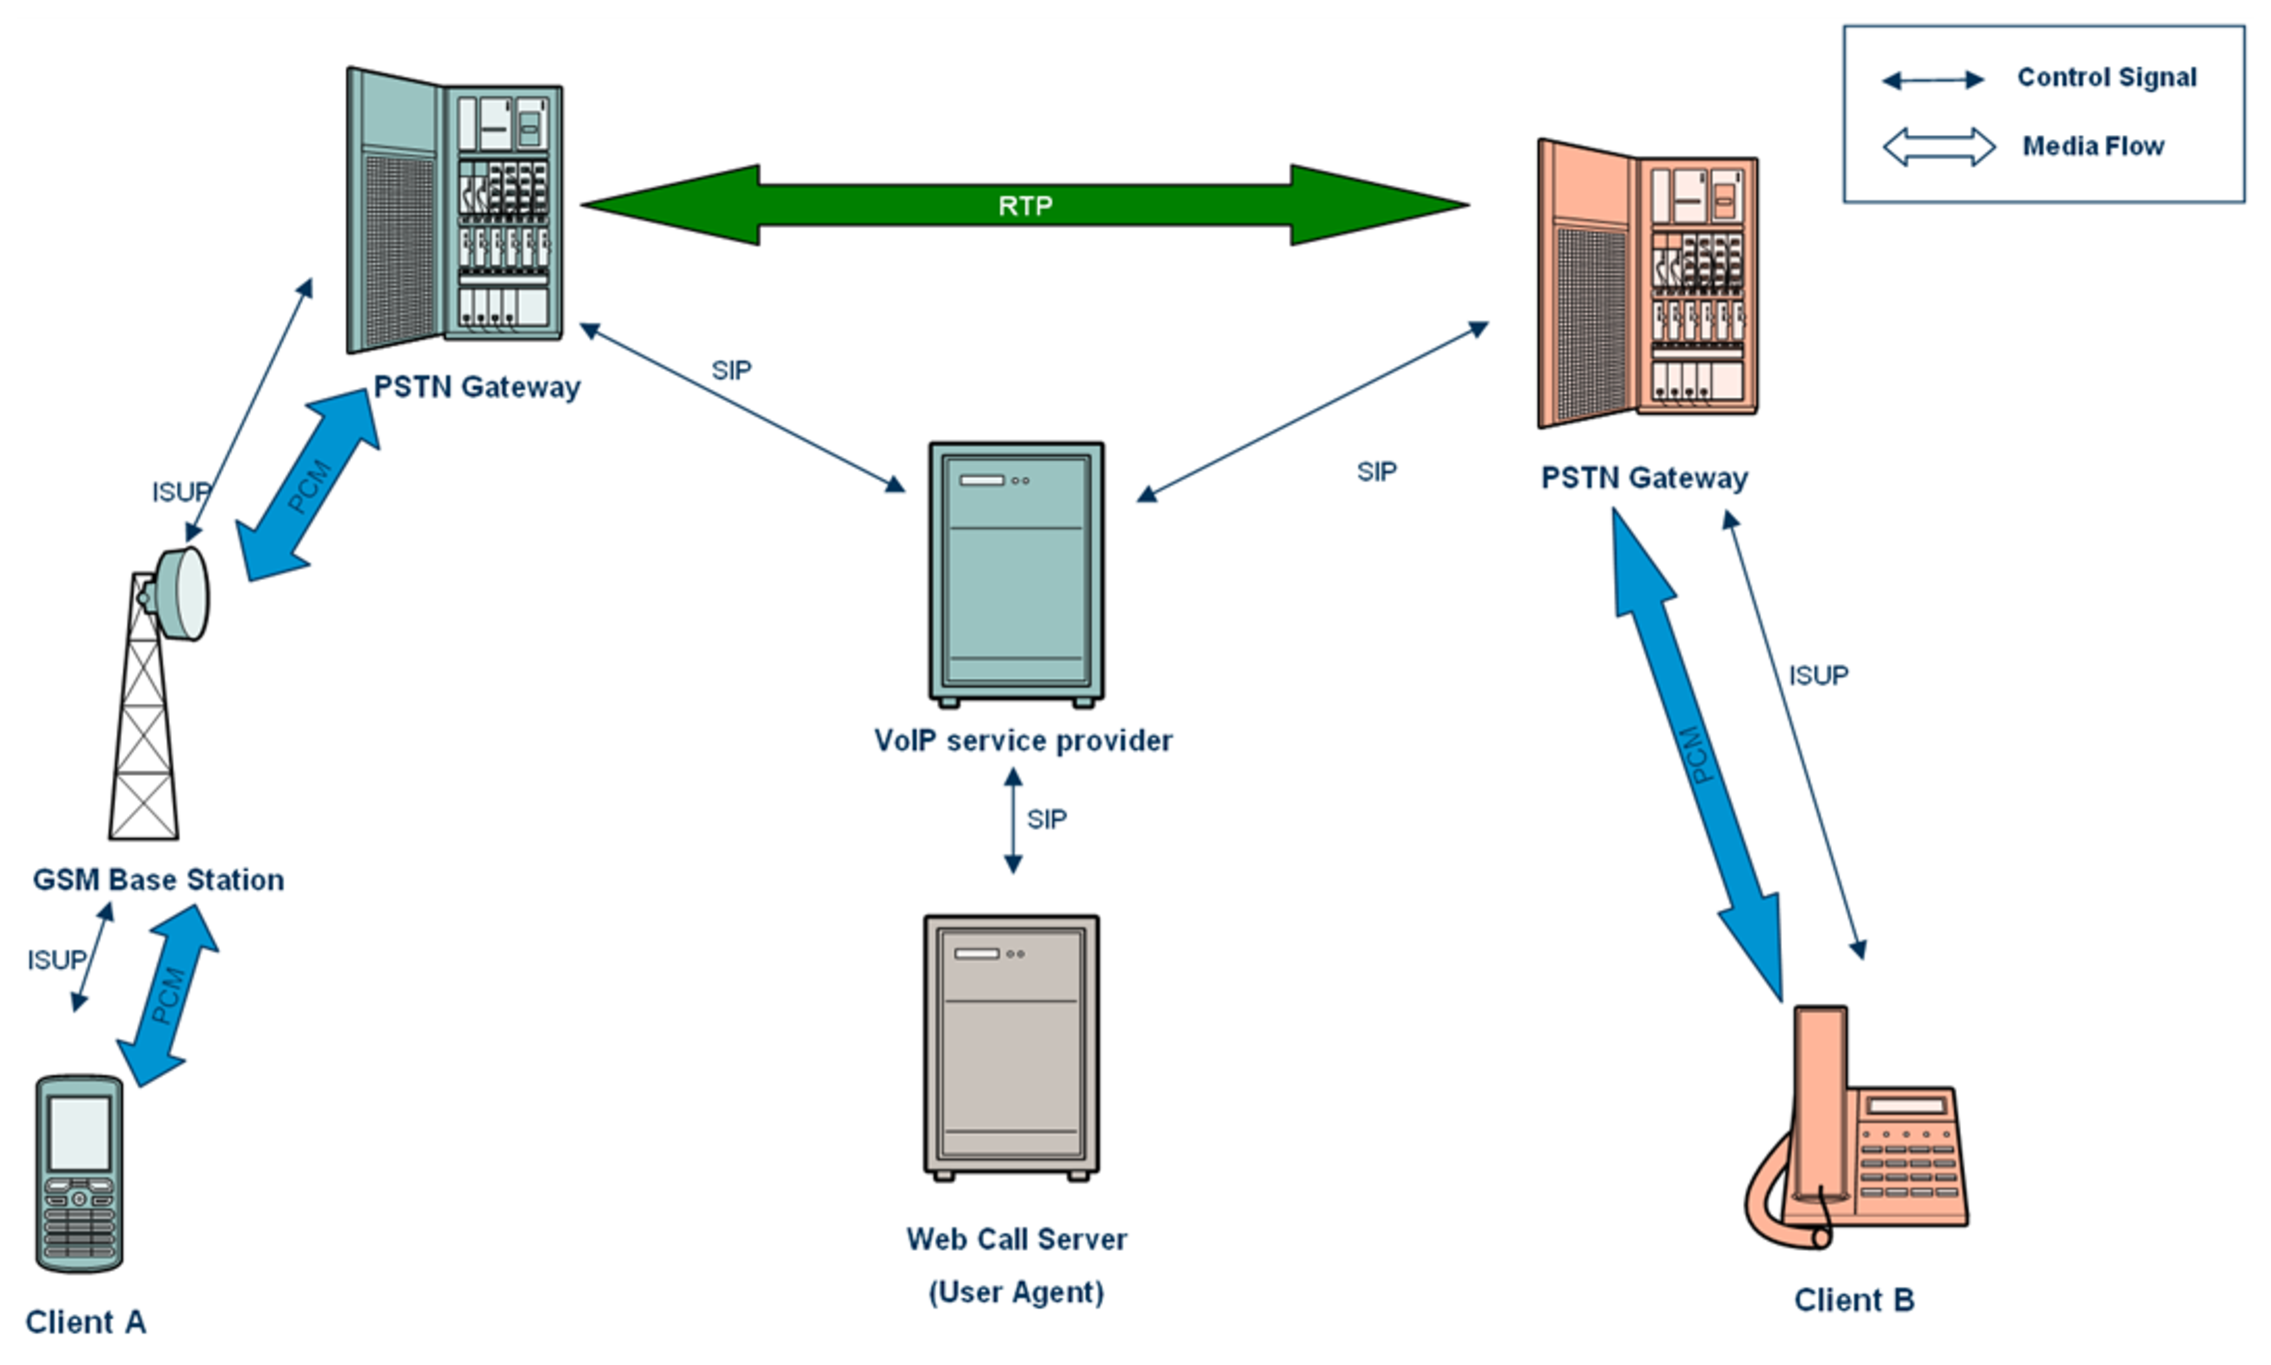
\epsfig{file=chap04/resources/the_signal_and_media_flow_of_3pc, width=5.34in}
\caption{The signal and media flow of Third Party Call}
\label{fig:TheSignalAndMediaFlowOf3pc}
\end{figure}




\subsection{Call Transfer}
\label{sec:Solution:ThirdPartyCall:CallTransfer}


\subsection{SDP Swap}
\label{sec:Solution:ThirdPartyCall:SDPSwep}

\subsection{Re-invite}
\label{sec:Solution:ThirdPartyCall:Re-invite}

\subsection{Web Client}
\label{sec:Solution:ThirdPartyCall:WebClient}


\section{Conclusion}
\label{sec:Solution:Conclusion}




% ********** End of chapter **********
